\documentclass[12pt]{article}
\usepackage{graphicx}
\usepackage{epstopdf}
  
%
% Title[Enter title of the experiment here]
\title{EE230: Experiment No.04\\
Opamps circuits-2\\}

% Author[Enter details of author here]
\author{Mudavath vishnuvardhan,200070044}

% begin the document.
\begin{document}

% make a title page.[this creates title page]
\maketitle

\section{Overview of the experiment} %[This segment creates Section as seen in document]

\subsection{Aim of the experiment}%[This segment creates sebsections under the same section]
Aim of this experiment is using Opamp to make half wave , full wave rectifier and improving them from that made using diodes (bridge rectifier).

\subsection{ Methods}

I used ngspice software to write code for schmitt trigger,astable multivibrator,monostable multivibrator and performed transient analysis, plotted time vs \(v_{in}\), \(v_{out}\) for all three circuits for different inputs and then extracted output files from each .cir ngspice file in .txt format and then used matplotlib to visualise this data from text file .
\newpage

\section{Design}%[To add multiple sections, keep appending blocks like this]

\subsection{Schmitt Trigger}

connect a 6v peak sinusodial voltage as shown below and measure \(v_{out}\).\\
for \(v_{in}=6sin(wt)\):\\
when \(v_{in}=v_{-}\) is lesser than \(v_{+}\),\(v_{out}\) goes to \(v_{th}\) similarly when it is greater than \(v_{-}\),\(v_{out}\) goes to \(-v_{th}\) because as \(v_{out}=A(v_{+}-v_{-})\) if \(v_{+}-v_{-}\) is slighlty positive too \(v_{out}\) goes to \(v_{th}\) because of multiplication of A which is large number and it happen commulatively. similar things happens for \(v_{a}=3v\),\(v_{a}=-3v\). where \(v_{th}=v_{0}R_{2}/(R_{1}+R_{2})\)\\
 \begin{figure}[h!]
\centering
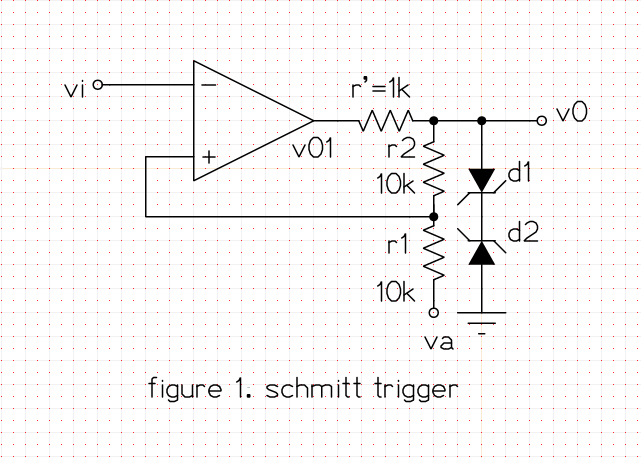
\includegraphics[scale = 0.6]{schmitt_trigger.png}
\end{figure}
\newpage

 
\subsection{Astable multivibrator}
The circuit for astable multivibrator is connected as shown in figure it has no external input.
then i perormed transient analysis. output of opamp produces nearly rectangular pulse because intially \(v_{+}>v_{-}\) thus \(v_{out}=v_{th}\) because of schmitt trigger effect therefore it charges capacitor for some time when voltage across input increases as it increases in rc circuit that is \(v_{c}=v_{o}(1-e^{-t/rc})\) ,when \(v_{out}\) becomes negative because as voltage across capacitor builds up  \(v_{+}<v_{-}\) thus \(v_{out}=-v_{th}\) ,tus voltage across capacitor becomes \(v_{c}=v_{o}(e^{-t/rc})\) that is voltage decreases exponentially.Where \(v_{th}=v_{0}R_{2}/(R_{1}+R_{2})\) \\

\begin{figure}[h!]
\centering
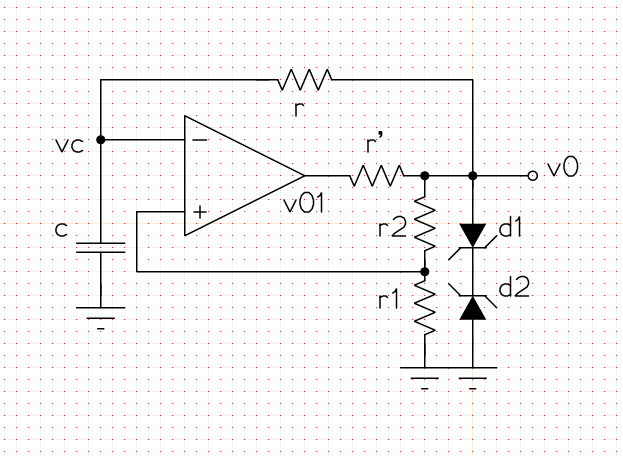
\includegraphics[scale = 0.6]{astable_multi.png}
\end{figure}
\newpage

\subsection{Monostable multivibrator}
connect the circuit for monostable multivibrator is shown below.when switch is closed the capacitor gets shorted thus input for inverting terminal for opamp becomes 15v as shown but when opened voltage across inverting terminal becomes voltage across a capacitor in a rc circuit that is \(v_{c}=v_{o}(1-e^{-t/rc})\) thus intially \(v_{-}\) becomes 0 slowly it starts building voltage ,thus intially as voltage across \(v_{+}\) greater than \(v_{-}\) thus \(v_{out}\) becomes \(v_{th}\) but as \(v_{-}\) increases it becomes greater than \(v_{+}\) eventually then \(v_{out}\) becomes \(-v_{th}\). Where \(v_{th}=v_{0}R_{2}/(R_{1}+R_{2})\).
\begin{figure}[h!]
\centering
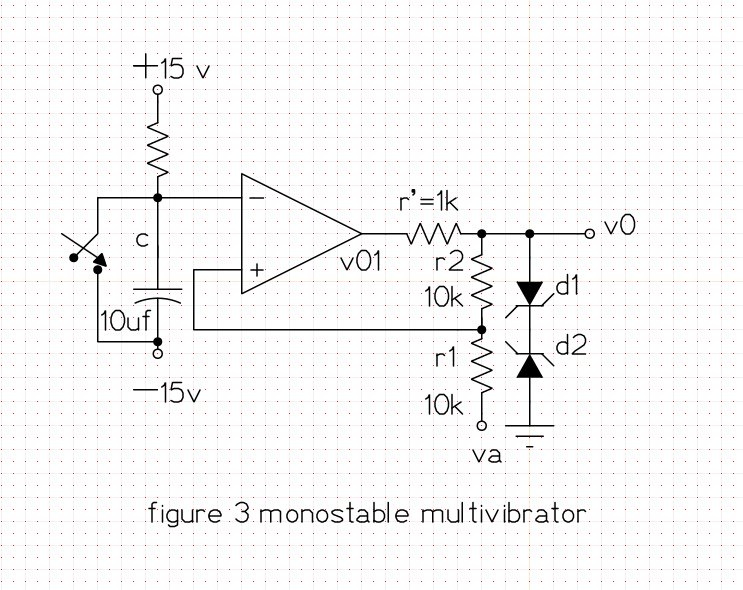
\includegraphics[scale = 0.4]{mono_multivib.png}
\end{figure}
\newpage

 
\section{Simulation results}%[One more section]
\subsection{Code snippet}

\subsubsection{schmitt trigger}
schmitt trigger circuit\\
.subckt ua741    1  2  3  4  5\\
c1   11 12 8.661E-12\\
c2    6  7 30.00E-12\\
dc    5 53 dx\\
de   54  5 dx\\
dlp  90 91 dx\\
dln  92 90 dx\\
dp    4  3 dx\\
egnd 99  0 poly(2) (3,0) (4,0) 0 .5 .5\\
fb    7 99 poly(5) vb vc ve vlp vln 0 10.61E6 -10E6 10E6 10E6 -10E6\\
ga    6  0 11 12 188.5E-6\\
gcm   0  6 10 99 5.961E-9\\
iee  10  4 dc 15.16E-6\\
hlim 90  0 vlim 1K\\
q1   11  2 13 qx\\
q2   12  1 14 qx\\
r2    6  9 100.0E3\\
rc1   3 11 5.305E3\\
rc2   3 12 5.305E3\\
re1  13 10 1.836E3\\
re2  14 10 1.836E3\\
ree  10 99 13.19E6\\
ro1   8  5 50\\
ro2   7 99 100\\
rp    3  4 18.16E3\\
vb    9  0 dc 0\\
vc    3 53 dc 1\\
ve   54  4 dc 1\\
vlim  7  8 dc 0\\
vlp  91  0 dc 40\\
vln   0 92 dc 40\\
.model dx D(Is=800.0E-18 Rs=1)\\
.model qx NPN(Is=800.0E-18 Bf=93.75)\\
.ends\\
\newpage
.subckt ZENER\_12 1 2\\
d1 1 2 df\\
dz 3 1 dr\\
vz 2 3 3.5\\
.model df D ( IS=27.5p RS=0.620 N=1.10 CJO=78.3p VJ=1.00 M=0.330 TT=50.1n)\\
.model dr D ( IS=5.49f RS=50 N=1.77 )\\
.ends\\
vin 1 0 sin(0 6 1k 0 0)\\
x1 5 1 6 7 2 ua741\\
ro 2 3 1k\\
r2 3 5 10k\\
r1 5 8 10k\\
va 8 0 -3v\\
x2 3 4 ZENER\_12\\
x3 0 4 ZENER\_12\\
vdd1 6 0 15v\\
vdd2 7 0 -15v\\
.tran 0.01u 4m\\
.control\\
run \\
plot v(3) v(1)\\
.endc\\
.end\\
\newpage


\subsubsection{Astable multivibrator}
\textbf{without r' and zener diode\\}
astable multivibrator\\
.subckt ua741    1  2  3  4  5\\
c1   11 12 8.661E-12\\
c2    6  7 30.00E-12\\
dc    5 53 dx\\
de   54  5 dx\\
dlp  90 91 dx\\
dln  92 90 dx\\
dp    4  3 dx\\
egnd 99  0 poly(2) (3,0) (4,0) 0 .5 .5\\
fb    7 99 poly(5) vb vc ve vlp vln 0 10.61E6 -10E6 10E6 10E6 -10E6\\
ga    6  0 11 12 188.5E-6\\
gcm   0  6 10 99 5.961E-9\\
iee  10  4 dc 15.16E-6\\
hlim 90  0 vlim 1K\\
q1   11  2 13 qx\\
q2   12  1 14 qx\\
r2    6  9 100.0E3\\
rc1   3 11 5.305E3\\
rc2   3 12 5.305E3\\
re1  13 10 1.836E3\\
re2  14 10 1.836E3\\
ree  10 99 13.19E6\\
ro1   8  5 50\\
ro2   7 99 100\\
rp    3  4 18.16E3\\
vb    9  0 dc 0\\
vc    3 53 dc 1\\
ve   54  4 dc 1\\
\newpage
vlim  7  8 dc 0\\
vlp  91  0 dc 40\\
vln   0 92 dc 40\\
.model dx D(Is=800.0E-18 Rs=1)\\
.model qx NPN(Is=800.0E-18 Bf=93.75)\\
.ends\\
x1 1 2 3 4 5 ua741\\
r2 5 1 35k\\
r1 1 0 30k \\
c1 2 0 0.01u\\
r 5 2 50k\\
vdd1 3 0 15v\\
vdd2 4 0 -15v\\
.tran 0.1u 10m\\
.control\\
run\\
plot v(2) v(5)\\
.endc\\
.end\\
\newpage
\textbf{with r' and zener diode\\}
astable multivibrator with r' and diodes\\
.subckt ua741    1  2  3  4  5\\
c1   11 12 8.661E-12\\
c2    6  7 30.00E-12\\
dc    5 53 dx\\
de   54  5 dx\\
dlp  90 91 dx\\
dln  92 90 dx\\
dp    4  3 dx\\
egnd 99  0 poly(2) (3,0) (4,0) 0 .5 .5\\
fb    7 99 poly(5) vb vc ve vlp vln 0 10.61E6 -10E6 10E6 10E6 -10E6\\
ga    6  0 11 12 188.5E-6\\
gcm   0  6 10 99 5.961E-9\\
iee  10  4 dc 15.16E-6\\
hlim 90  0 vlim 1K\\
q1   11  2 13 qx\\
q2   12  1 14 qx\\
r2    6  9 100.0E3\\
rc1   3 11 5.305E3\\
rc2   3 12 5.305E3\\
re1  13 10 1.836E3\\
re2  14 10 1.836E3\\
ree  10 99 13.19E6\\
ro1   8  5 50\\
ro2   7 99 100\\
rp    3  4 18.16E3\\
vb    9  0 dc 0\\
vc    3 53 dc 1\\
ve   54  4 dc 1\\
vlim  7  8 dc 0\\
vlp  91  0 dc 40\\
vln   0 92 dc 40\\
.model dx D(Is=800.0E-18 Rs=1)\\
.model qx NPN(Is=800.0E-18 Bf=93.75)\\
.ends\\
\newpage
.subckt ZENER\_12 1 2\\
d1 1 2 df\\
dz 3 1 dr\\
vz 2 3 3.5\\
.model df D ( IS=27.5p RS=0.620 N=1.10 CJO=78.3p VJ=1.00 M=0.330 TT=50.1n)\\
.model dr D ( IS=5.49f RS=50 N=1.77 )\\
.ends\\
x1 1 2 3 4 5 ua741\\
rd 5 6 1k\\
r2 6 1 35k\\
r1 1 0 30k \\
c1 2 0 0.01u\\
r 6 2 50k\\
x2 6 7 ZENER_12\\
x3 0 7 ZENER_12\\
vdd1 3 0 15v\\
vdd2 4 0 -15v\\
.tran 0.1u 10m\\
.control\\
run\\
plot v(2) v(5) v(6)\\
.endc\\
.end\\
\newpage


\subsubsection{Monostable multivibrator}
monostable multivibrator part a\\
.subckt ua741    1  2  3  4  5\\
c1   11 12 8.661E-12\\
c2    6  7 30.00E-12\\
dc    5 53 dx\\
de   54  5 dx\\
dlp  90 91 dx\\
dln  92 90 dx\\
dp    4  3 dx\\
egnd 99  0 poly(2) (3,0) (4,0) 0 .5 .5\\
fb    7 99 poly(5) vb vc ve vlp vln 0 10.61E6 -10E6 10E6 10E6 -10E6\\
ga    6  0 11 12 188.5E-6\\
gcm   0  6 10 99 5.961E-9\\
iee  10  4 dc 15.16E-6\\
hlim 90  0 vlim 1K\\
q1   11  2 13 qx\\
q2   12  1 14 qx\\
r2    6  9 100.0E3\\
rc1   3 11 5.305E3\\
rc2   3 12 5.305E3\\
re1  13 10 1.836E3\\
re2  14 10 1.836E3\\
ree  10 99 13.19E6\\
ro1   8  5 50\\
ro2   7 99 100\\
rp    3  4 18.16E3\\
vb    9  0 dc 0\\
vc    3 53 dc 1\\
ve   54  4 dc 1\\
\newpage
vlim  7  8 dc 0\\
vlp  91  0 dc 40\\
vln   0 92 dc 40\\
.model dx D(Is=800.0E-18 Rs=1)\\
.model qx NPN(Is=800.0E-18 Bf=93.75)\\
.ends\\
.subckt ZENER\_12 1 2\\
d1 1 2 df\\
dz 3 1 dr\\
vz 2 3 3.5\\
.model df D ( IS=27.5p RS=0.620 N=1.10 CJO=78.3p VJ=1.00 M=0.330 TT=50.1n)\\
.model dr D ( IS=5.49f RS=50 N=1.77 )\\
.ends\\
.subckt button\_sw 1 2\\
s1 1 2 c 0 b\_sw1\\
v1 c 0 pulse(0 10 0.10 0.02 0.02 0.05 100)\\
.model b\_sw1 sw vt=1 vh=0.2 ron=1 roff=1000MEG\\
.ends\\
\newpage
x1 1 2 3 4 5 ua741\\
x2 2 6 button_sw\\
v1 6 0 -15v\\
c1 2 6 10u\\
r 2 7 10k\\
v2 7 0 15v\\
v3 3 0 15v\\
v4 4 0 -15v\\
rd 5 8 1k\\
r2 8 1 10k\\
r1 1 0 10k\\
x3 8 9 ZENER\_12\\
x4 0 9 ZENER\_12\\
.tran 0.1m 2s\\
.control\\
run\\
plot v(8)\\
plot v(2) v(8) v(2)-v(6)\\
.endc\\
.end\\
\newpage


\subsection{Simulation results}
\subsubsection{schmitt trigger}
\textbf{Va=gnd\\}
X-axis is time axis, Y-axis is voltage axis time vs \(V_{in}\), \(V_{out}\) is plotted below . plot shows that when \(V_{in}\) is sinusodial \(V_{out}\) becomes nearly rectangular wave of amplitude +5.8v and -5.8v and frequency 900 Hz .\\
\begin{figure}[h!]
\centering
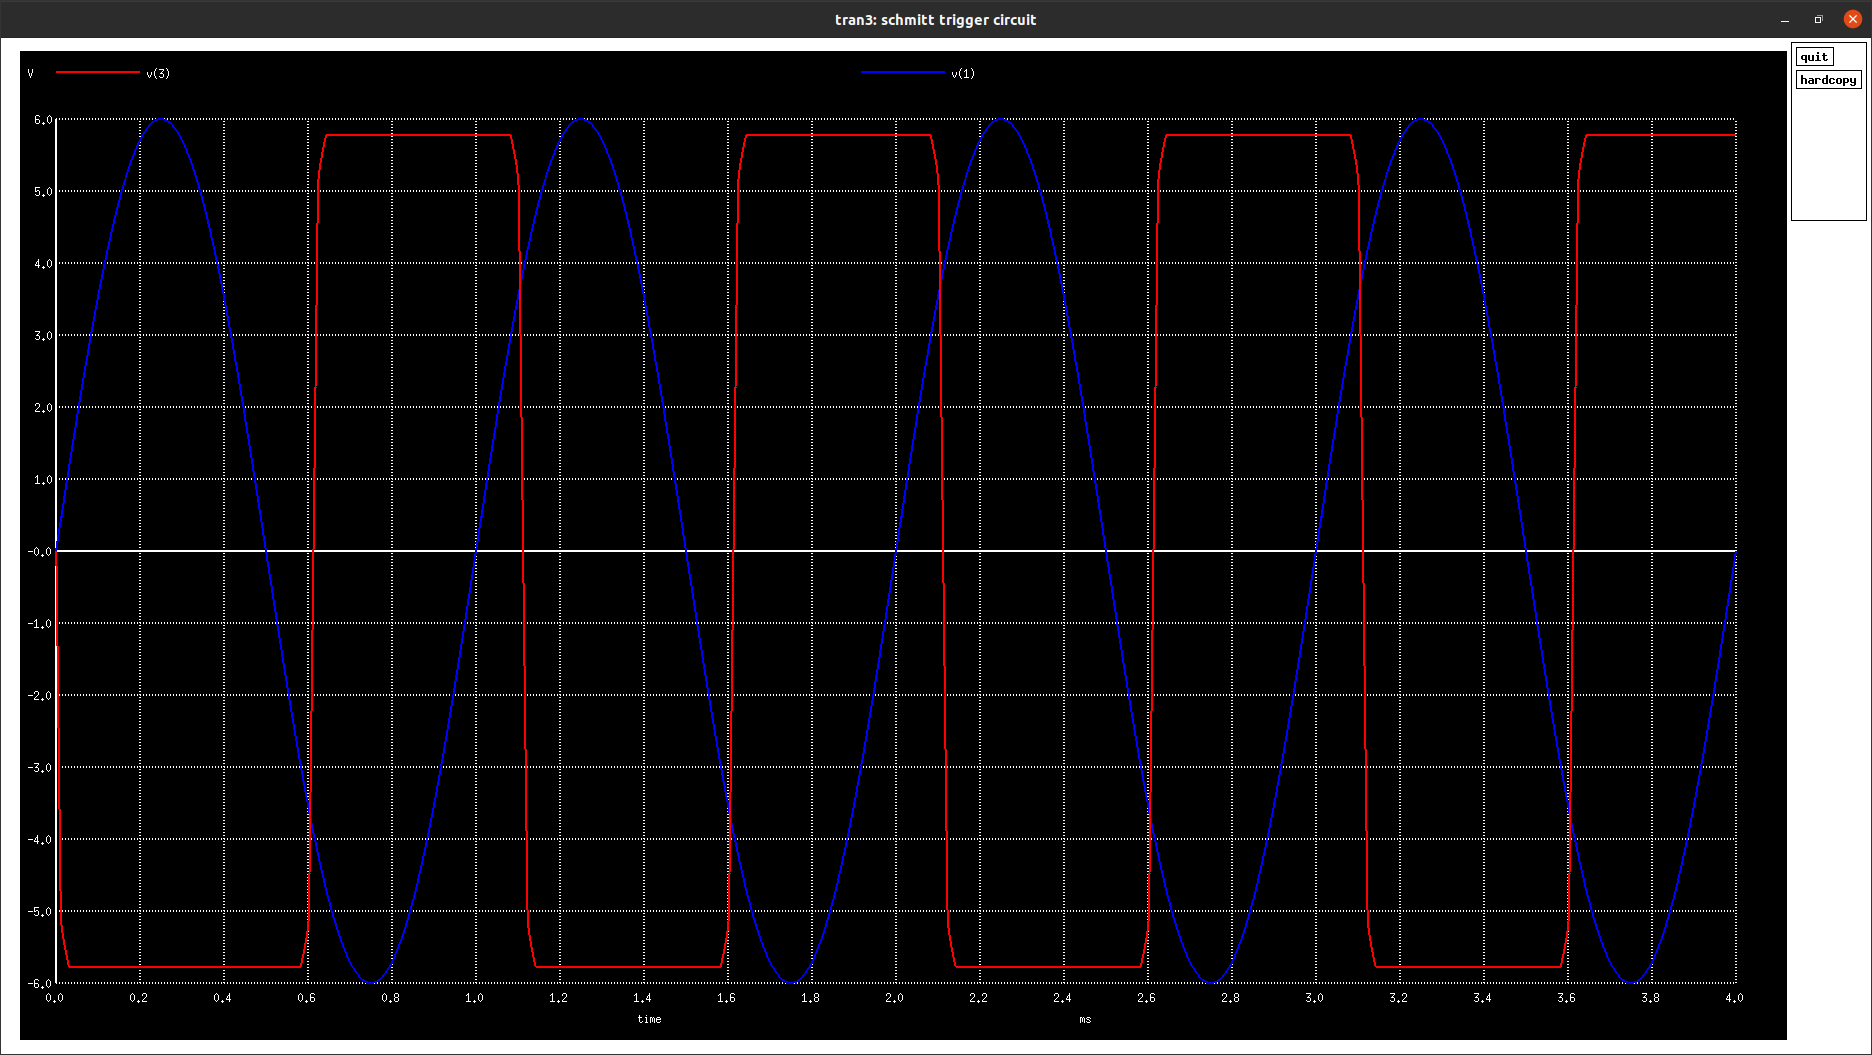
\includegraphics[scale = 0.2]{q1_gnd_sin.png}
\end{figure}
\newpage
\begin{figure}[h!]
\centering
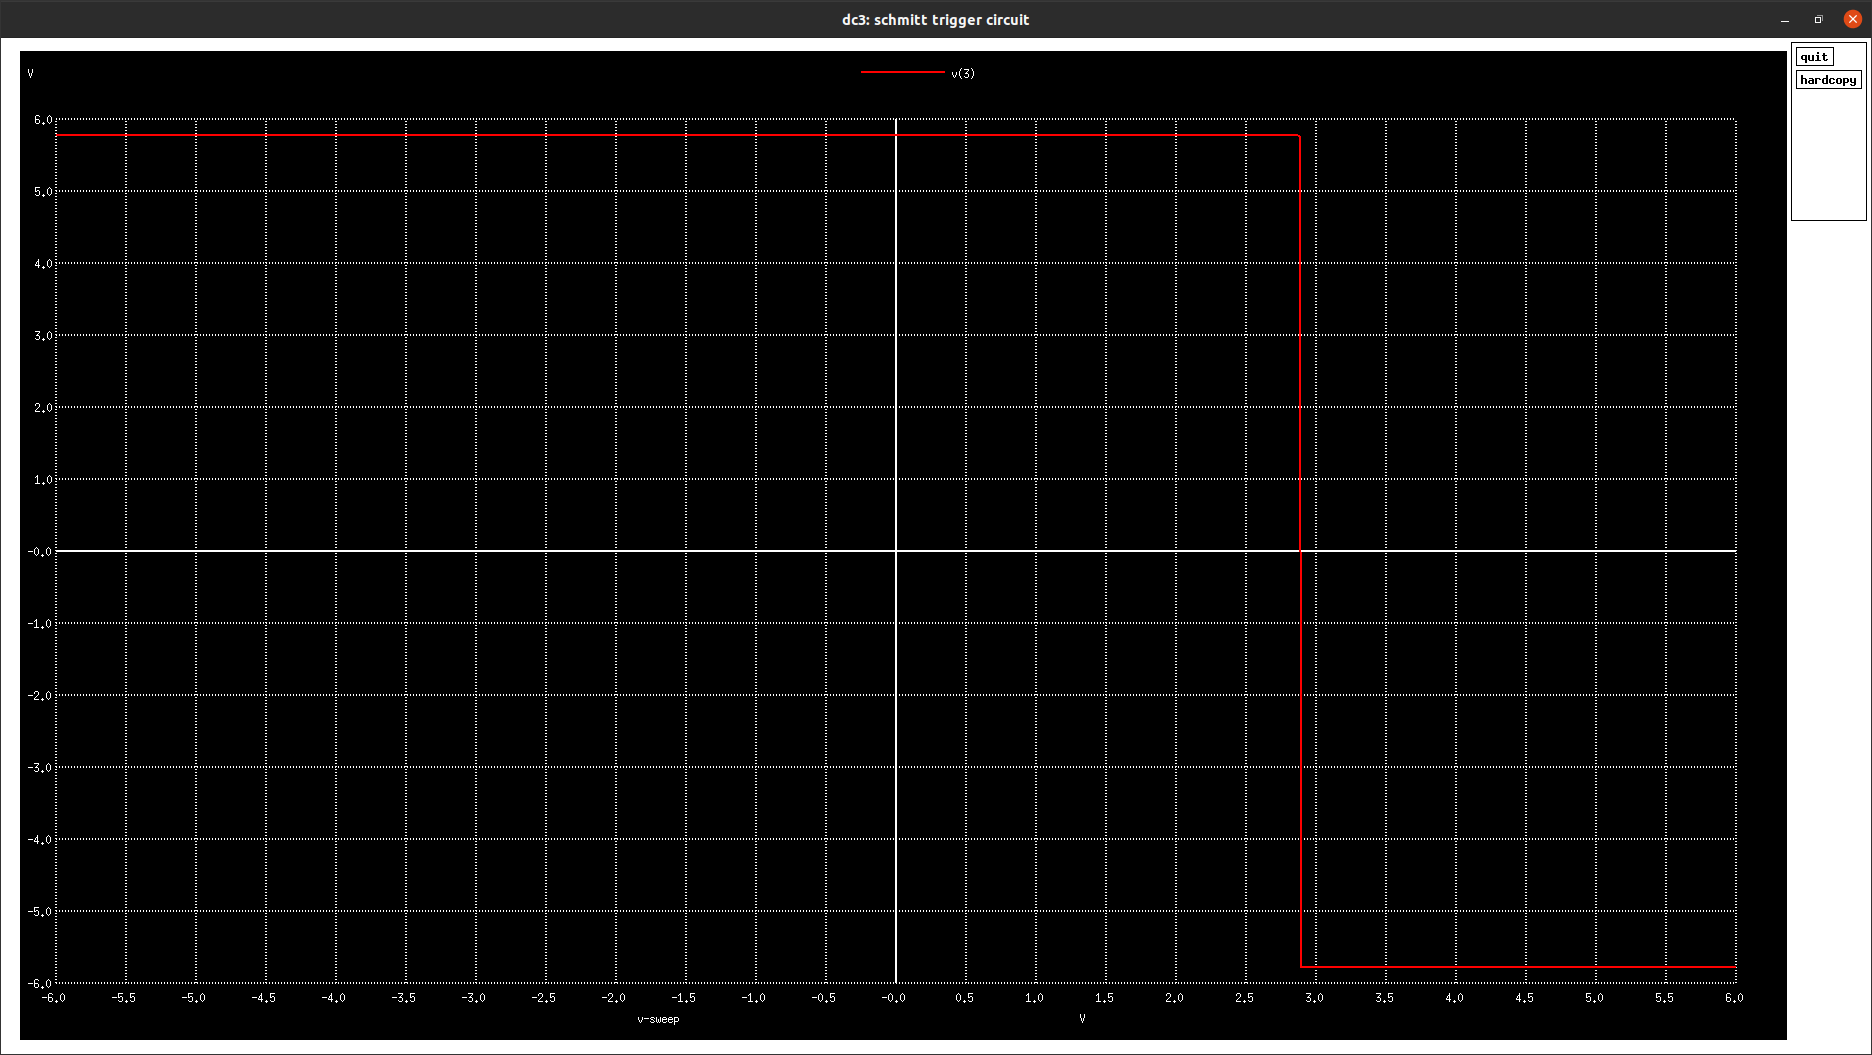
\includegraphics[scale = 0.2]{q1_gnd_dc.png}
\end{figure}
\newpage

\textbf{Va=3v\\}
X-axis is time axis, Y-axis is voltage axis time vs \(V_{in}\), \(V_{out}\) is plotted below . plot shows that when \(V_{in}\) is sinusodial \(V_{out}\) becomes nearly rectangular wave of amplitude +5.8v and -5.8v and frequency 1000 Hz .\\
\begin{figure}[h!]
\centering
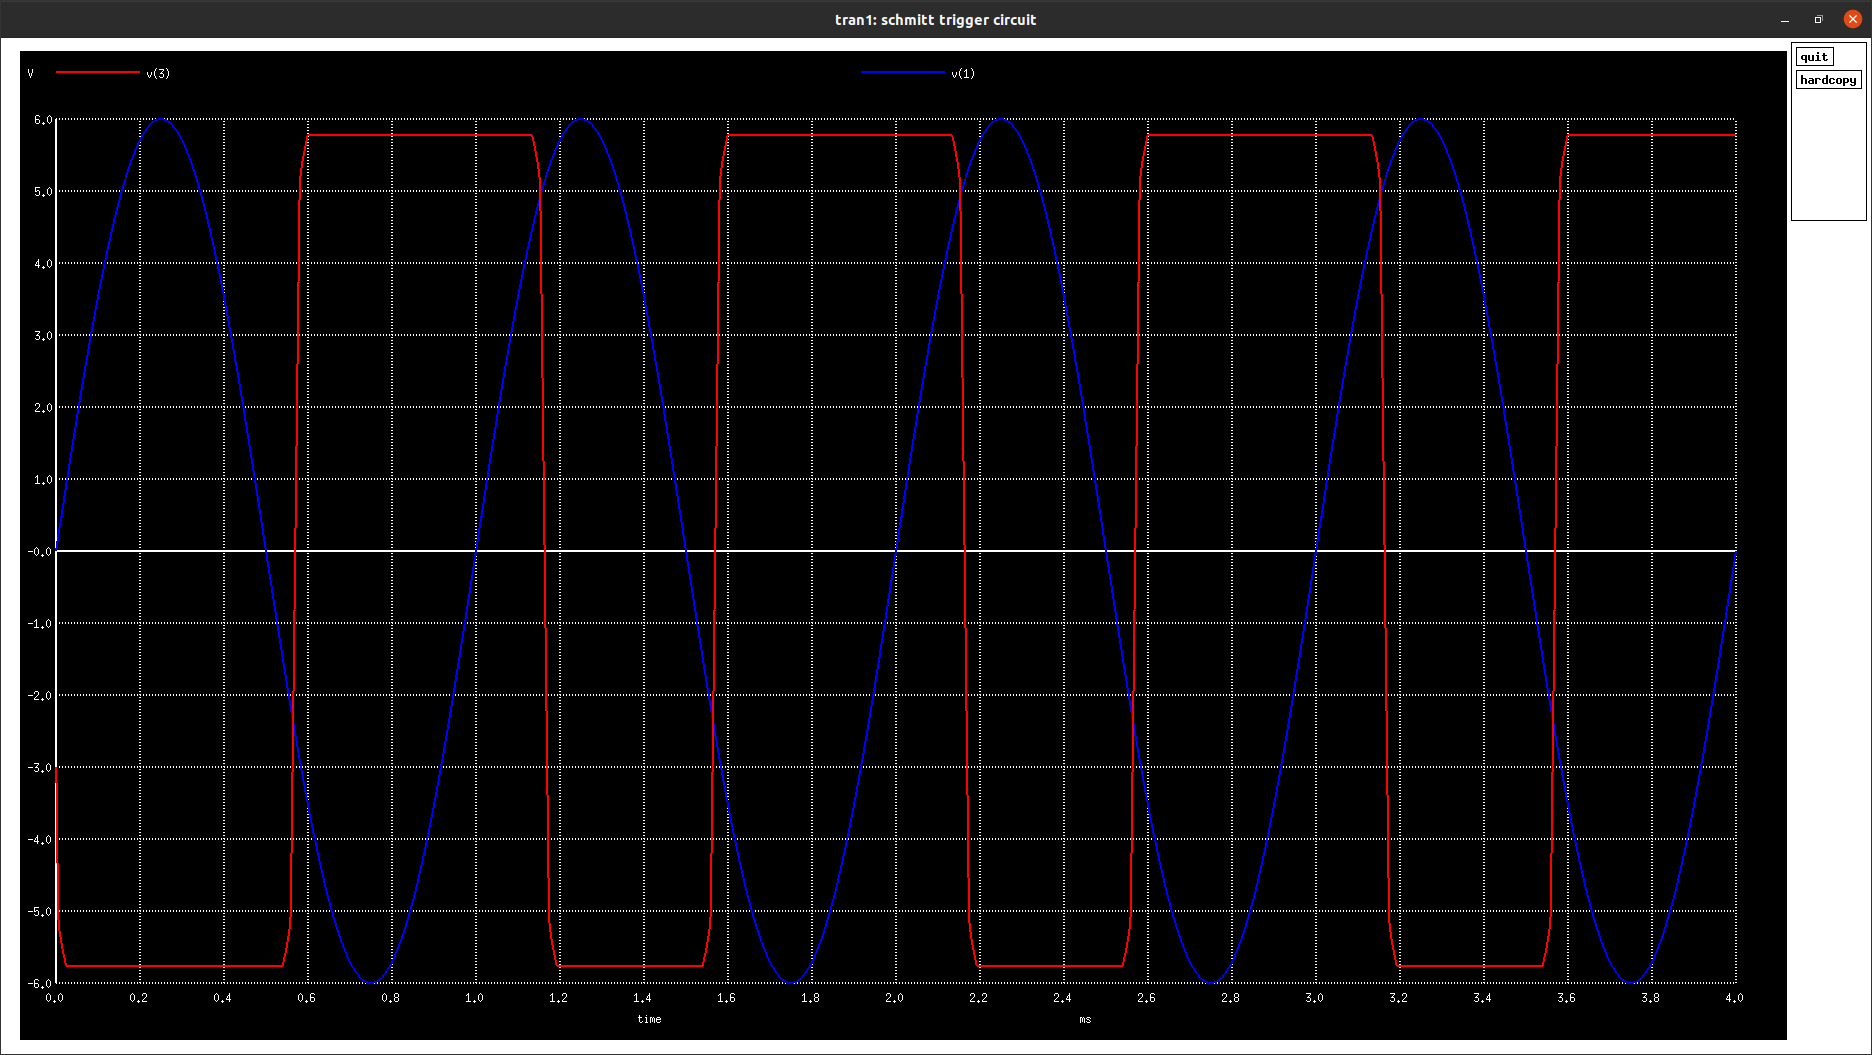
\includegraphics[scale = 0.2]{q1_3_sin.png}
\end{figure}
\newpage
\begin{figure}[h!]
\centering
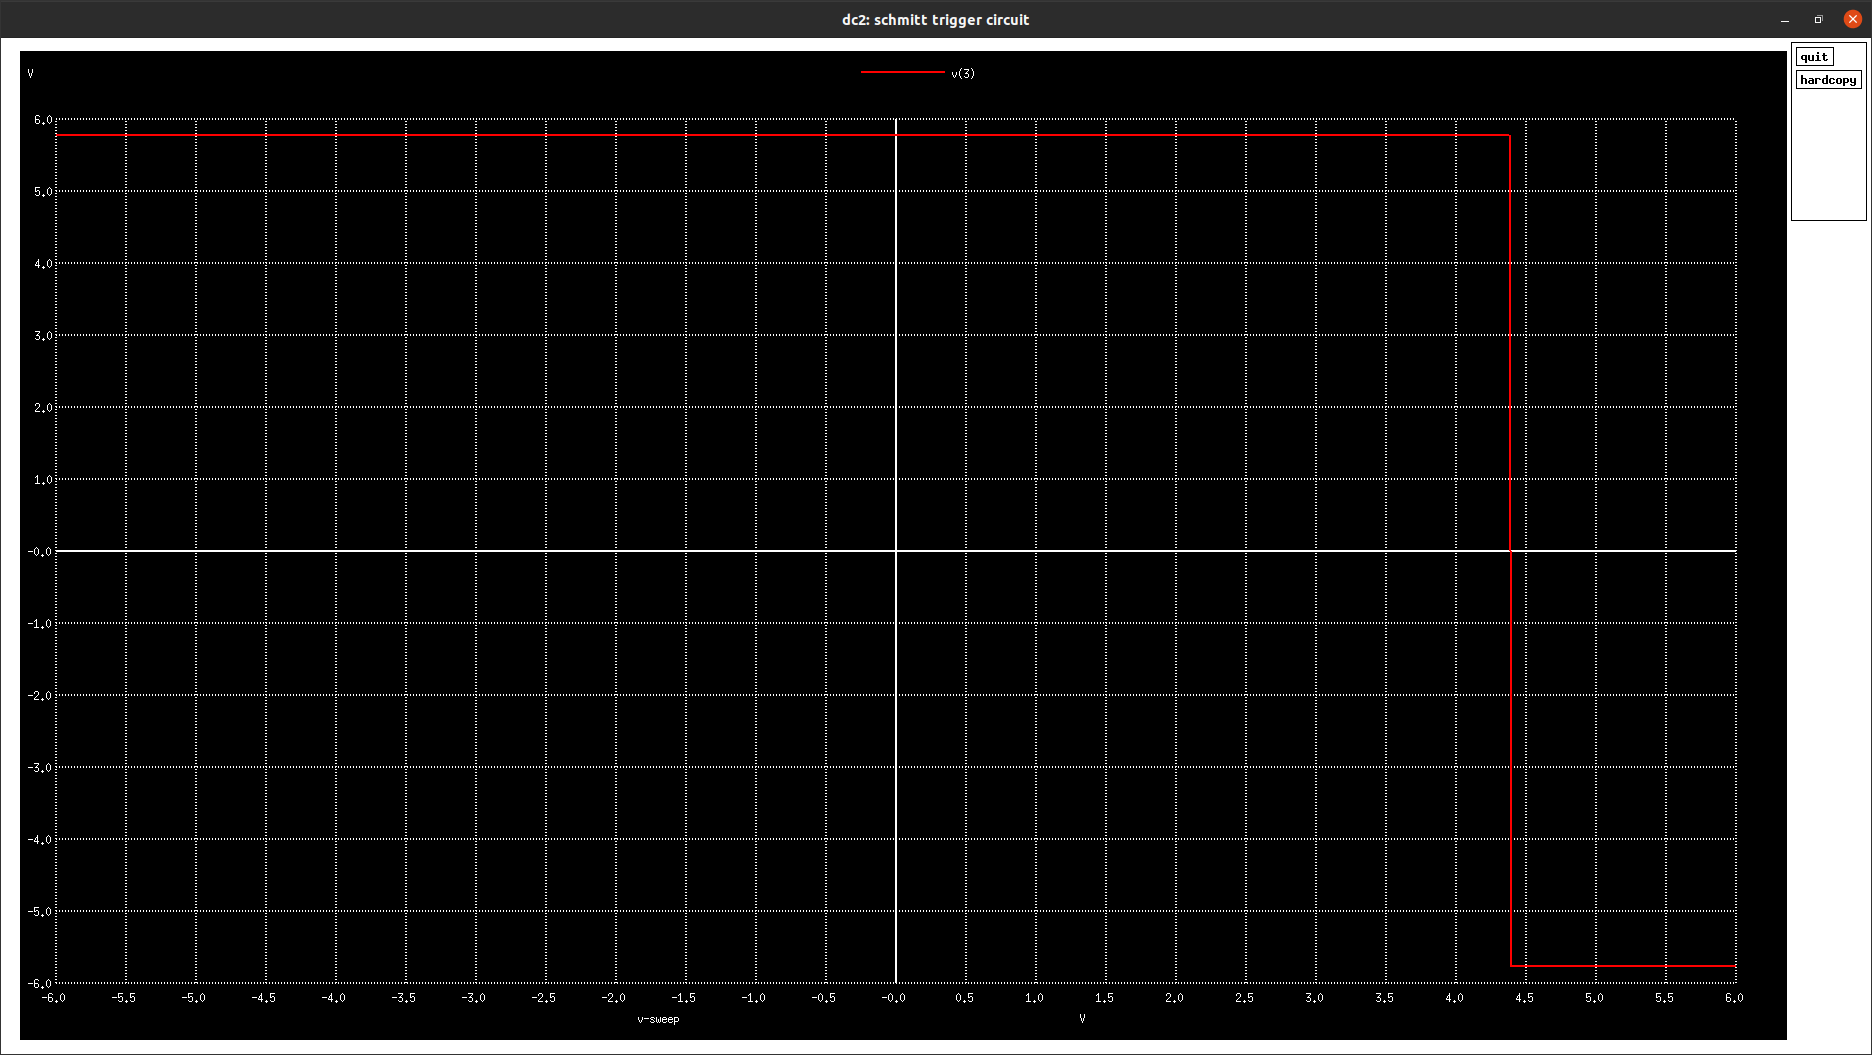
\includegraphics[scale = 0.2]{q1_3_dc.png}
\end{figure}
\newpage

\textbf{Va=-3v\\}
X-axis is time axis, Y-axis is voltage axis time vs \(V_{in}\), \(V_{out}\) is plotted below . plot shows that when \(V_{in}\) is sinusodial \(V_{out}\) becomes nearly rectangular wave of amplitude +5.8v and -5.8v and frequency 1000 Hz .\\
\begin{figure}[h!]
\centering
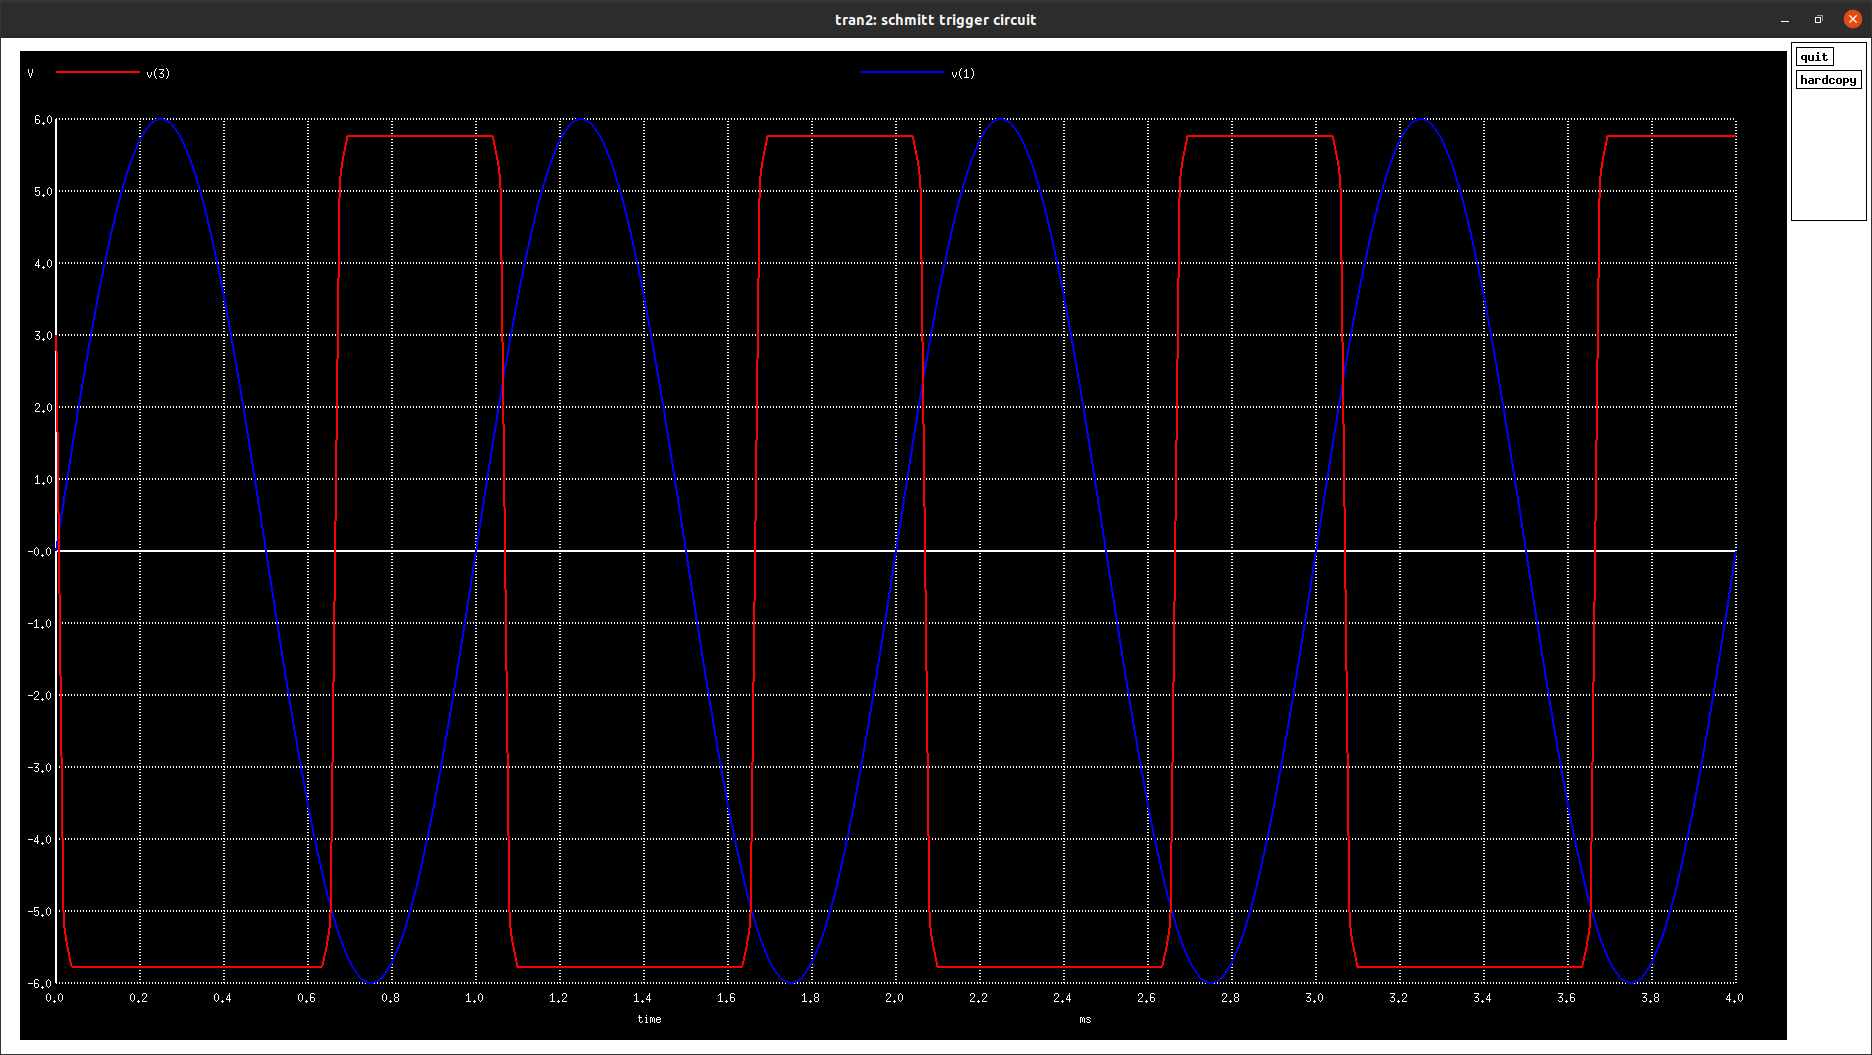
\includegraphics[scale = 0.2]{q1_-3_sin.png}
\end{figure}
\newpage
\begin{figure}[h!]
\centering
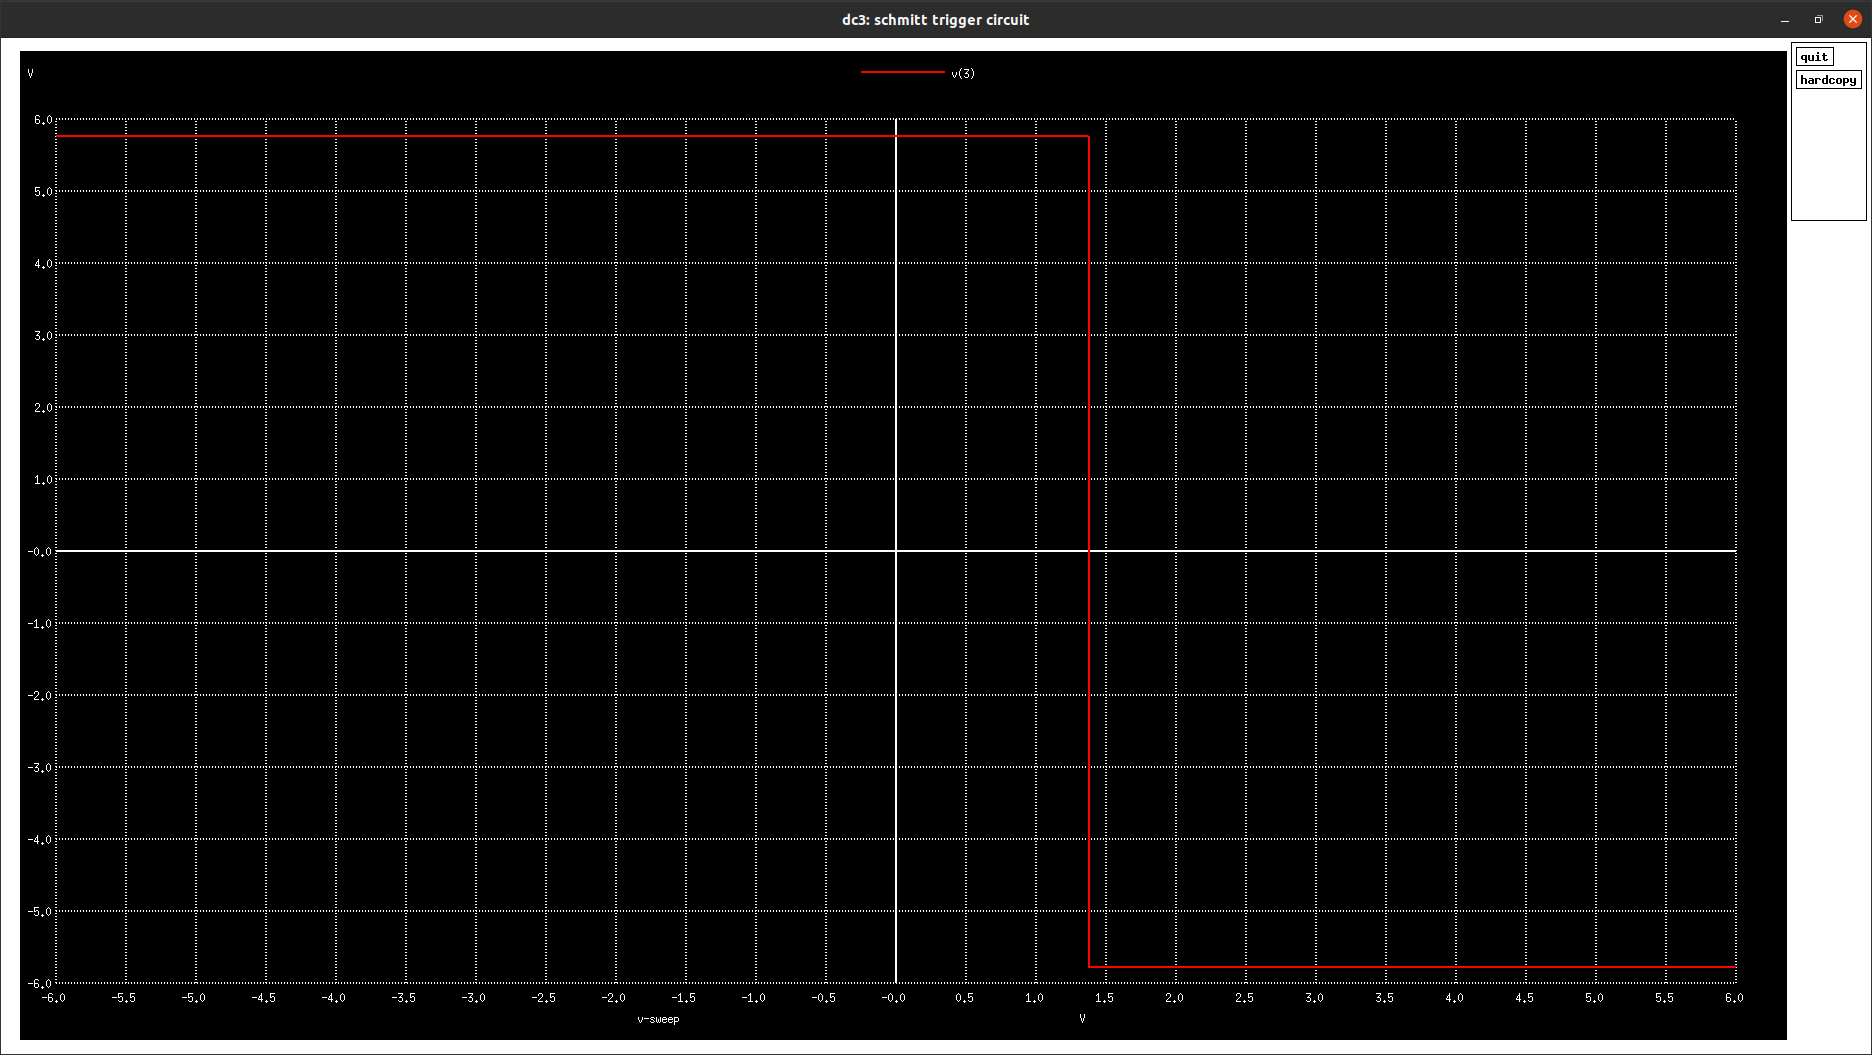
\includegraphics[scale = 0.2]{q1_-3_dc.png}
\end{figure}
\newpage


\subsubsection{astable multivibrator}
\textbf{with no r' and diode\\}
X-axis is time axis, Y-axis is voltage axis time vs \(V_{in}\), \(V_{out}\) is plotted below . plot shows that \(V_{in}\) increases with \(V_{out}=v_{th}\) and decreases with \(V_{out}=-v_{th}\). Frequency of this plot is 952 Hz.
\begin{figure}[h!]
\centering
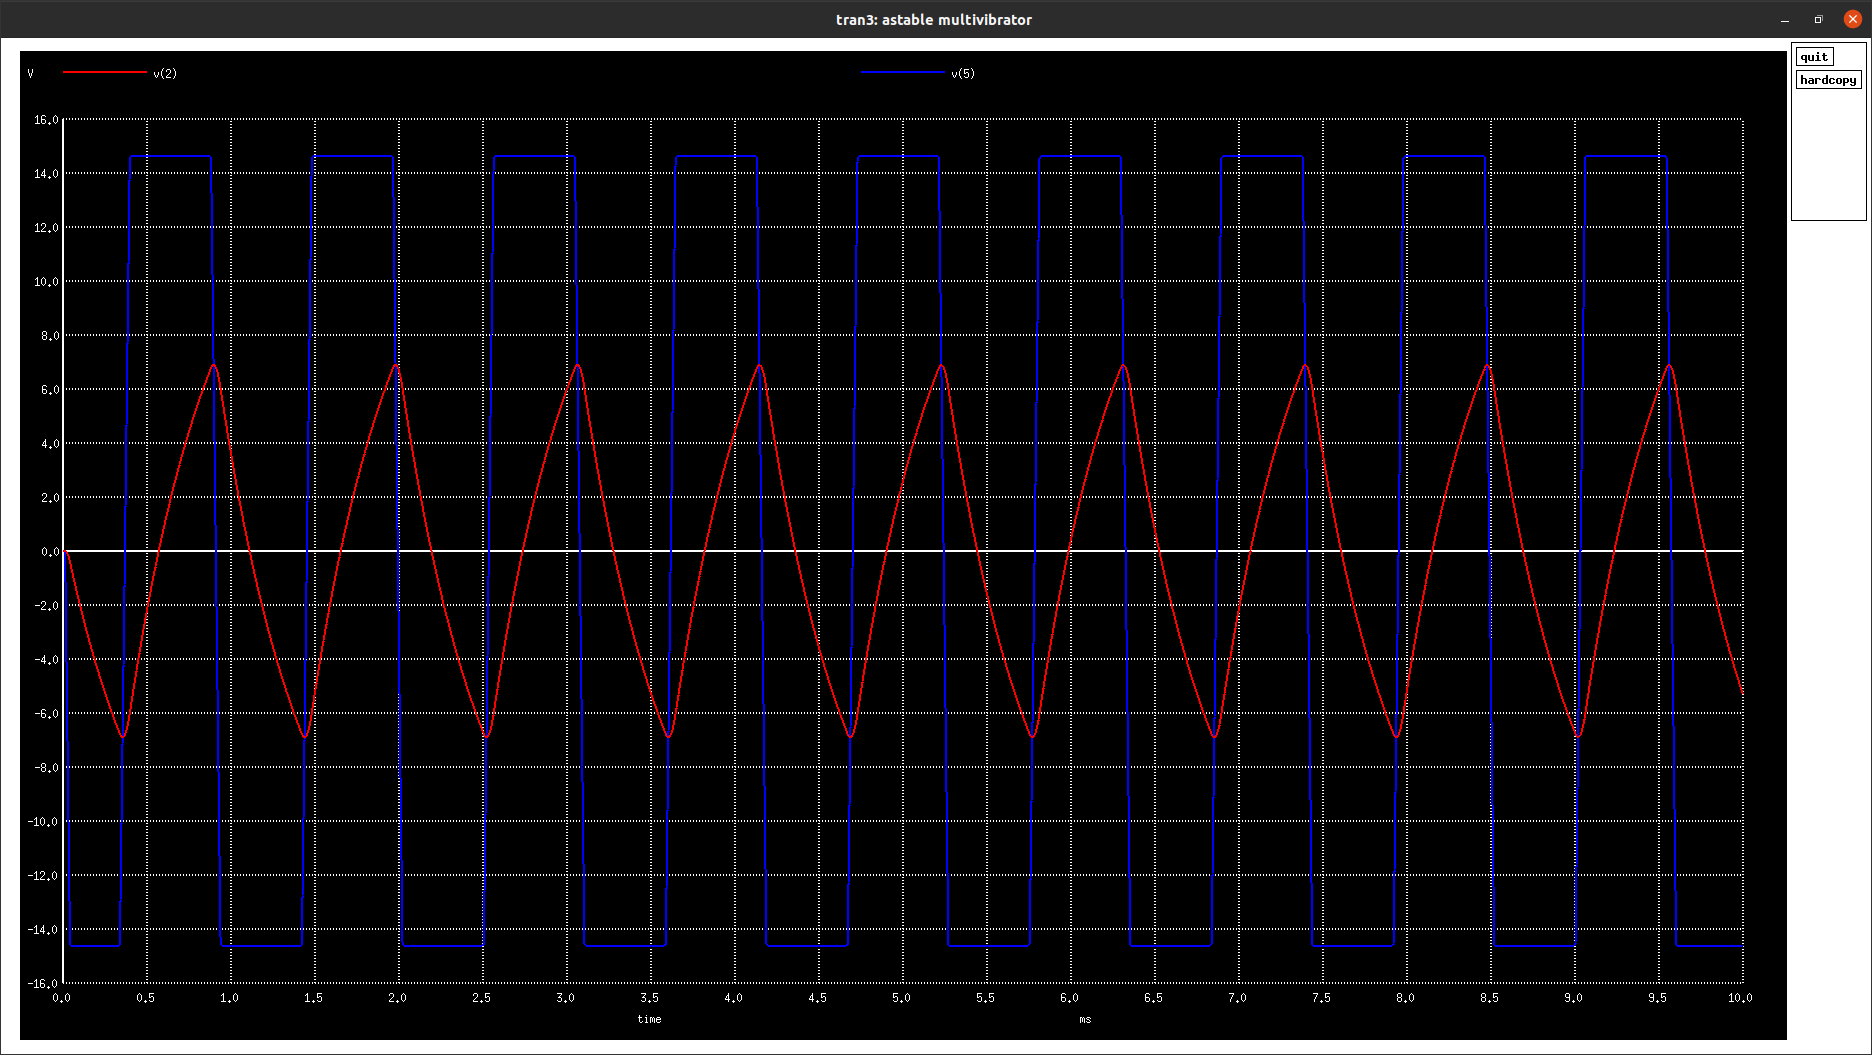
\includegraphics[scale = 0.2]{q2_nrd.png}
\end{figure}
\newpage
\textbf{with r' and diode\\}
X-axis is time axis, Y-axis is voltage axis time vs \(V_{in}\), \(V_{out}\) is plotted below . plot shows that \(V_{in}\) increases with \(V_{out}=v_{th}\) and decreases with \(V_{out}=-v_{th}\). Frequency of this plot is 909 Hz.
\begin{figure}[h!]
\centering
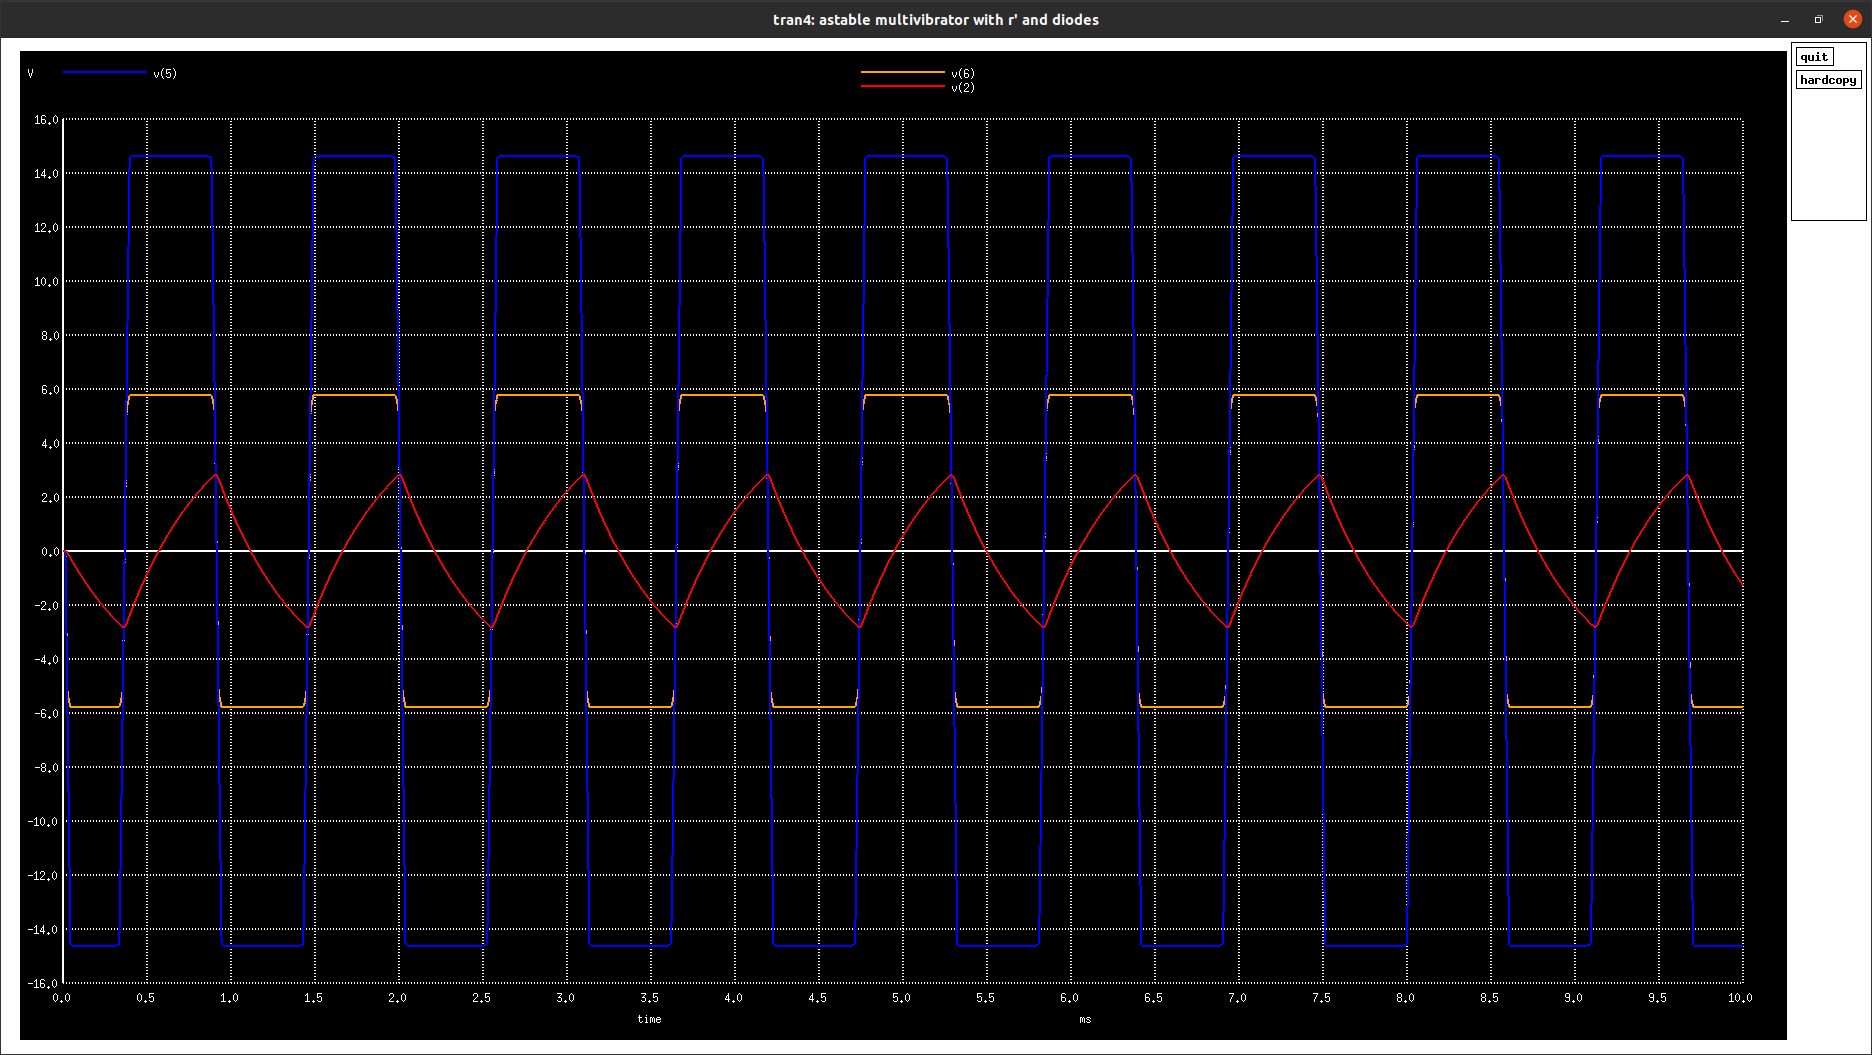
\includegraphics[scale = 0.2]{q2_rd.png}
\end{figure}
\newpage

\subsubsection{Monostable multivibrator}
X-axis is time axis, Y-axis is voltage axis time vs \(V_{in}\), \(V_{out}\) is plotted below . plot shows that intially \(V_{in}\) is 15v as it is shorted thus \(V_{out}\) becomes \(-V_{th}\)  but as switch is opened \(V_{in}\) becomes 0 thus \(V_{out}\) becomes \(V_{th}\)  and capacitor charges and as \(V_{in}\) increases \(V_{out}\) becomes \(-V_{th}\). Thus width of plot should be nearly equal to 0.18 seconds.
\begin{figure}[h!]
\centering
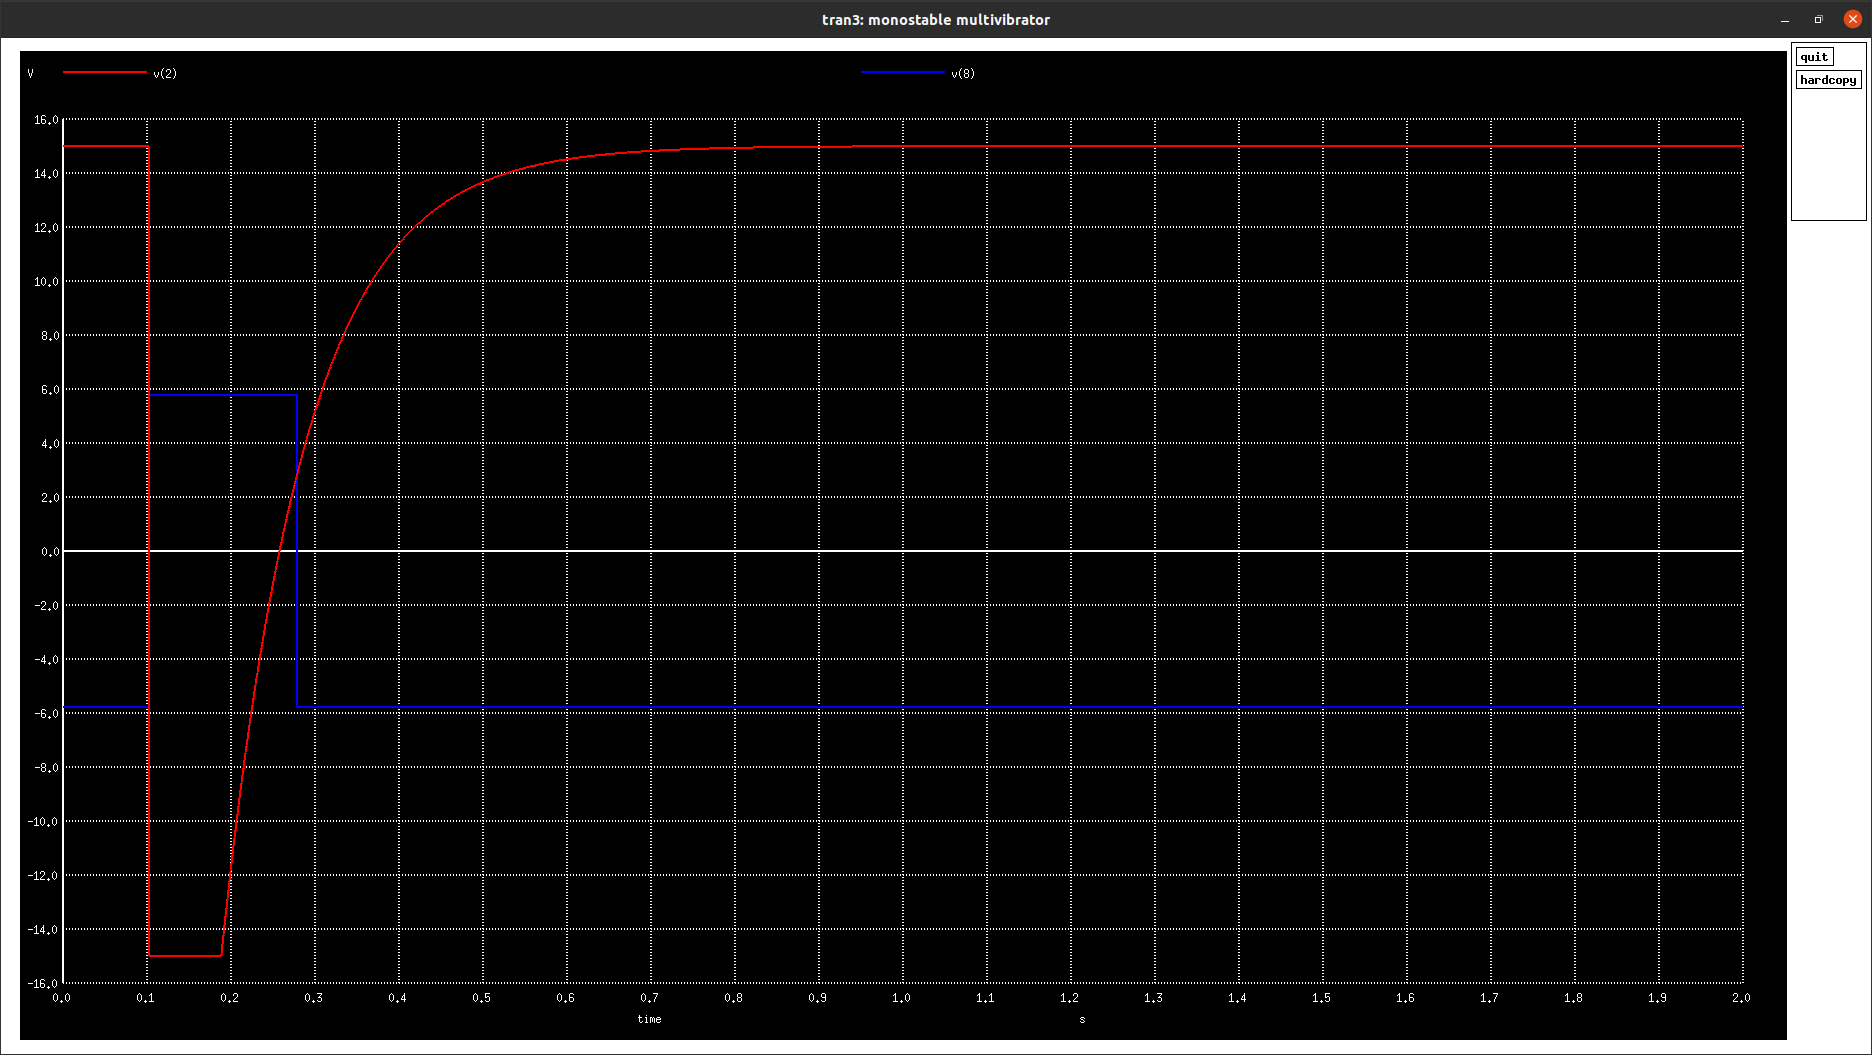
\includegraphics[scale = 0.2]{q3.png}
\end{figure}
\newpage

\section{Experiment completion status}
I have completed all sections in Lab only.

\end{document}
